\documentclass[12pt]{article}
\usepackage{amsmath}
\usepackage{graphicx}
\usepackage{hyperref}
\usepackage{listings}
\usepackage{color}
\usepackage{pythonhighlight}
\usepackage{multirow}
\usepackage{array}
\usepackage{graphicx}
\usepackage{xcolor}
\usepackage{amsmath}
\usepackage{float}


\title{Operating System Course Report - First Half of the Semester}
\author{A class}
\date{\today}

\begin{document}

\maketitle
\newpage

\tableofcontents
\newpage

\section{Introduction}
This report summarizes the topics covered during the first half of the Operating System course. It includes theoretical concepts, practical implementations, and assignments. The course focuses on the fundamentals of operating systems, including system architecture, process management, CPU scheduling, and deadlock handling.

\section{Course Overview}
\subsection{Objectives}
The main objectives of this course are:
\begin{itemize}
    \item To understand the basic components and architecture of a computer system.
    \item To learn process management, scheduling, and inter-process communication.
    \item To explore file systems, input/output management, and virtualization.
    \item To study the prevention and handling of deadlocks in operating systems.
\end{itemize}

\subsection{Course Structure}
The course is divided into two halves. This report focuses on the first half, which covers:
\begin{itemize}
    \item Basic Concepts and Components of Computer Systems
    \item System Performance and Metrics
    \item System Architecture of Computer Systems
    \item Process Description and Control
    \item Scheduling Algorithms
    \item Process Creation and Termination
    \item Introduction to Threads
    \item File Systems
    \item Input and Output Management
    \item Deadlock Introduction and Prevention
    \item User Interface Management
    \item Virtualization in Operating Systems
\end{itemize}
\section{Topics Covered}

\subsection{Basic Concepts and Components of Computer Systems}
This section explains the fundamental components that make up a computer system, including the CPU, memory, storage, and input/output devices.

\subsection{System Performance and Metrics}
This section introduces various system performance metrics used to measure the efficiency of a computer system, including throughput, response time, and utilization.

\subsection{System Architecture of Computer Systems}
Describes the architecture of modern computer systems, focusing on the interaction between hardware and the operating system.

\subsection{Process Description and Control}
Processes are a central concept in operating systems. This section covers:
\begin{itemize}
    \item Process states and state transitions
    \item Process control block (PCB)
    \item Context switching
\end{itemize}

\subsection{Scheduling Algorithms}
This section covers:
\begin{itemize}
    \item First-Come, First-Served (FCFS)
    \item Shortest Job Next (SJN)
    \item Round Robin (RR)
\end{itemize}
It explains how these algorithms are used to allocate CPU time to processes.

\subsection{Process Creation and Termination}
Details how processes are created and terminated by the operating system, including:
\begin{itemize}
    \item Process spawning
    \item Process termination conditions
\end{itemize}

\subsection{Introduction to Threads}
This section introduces the concept of threads and their relation to processes, covering:
\begin{itemize}
    \item Single-threaded vs. multi-threaded processes
    \item Benefits of multithreading
\end{itemize}

\begin{figure}[h]
    \centering
    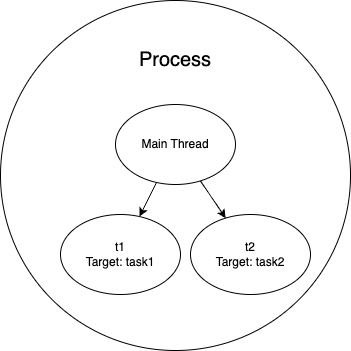
\includegraphics[width=0.5\textwidth]{../a_class/asset/example.png}  % Sesuaikan nama file dan ukurannya
    \caption{Ini adalah gambar contoh dari multithreading.}
    \label{fig:contoh_gambar}
\end{figure}
Seperti yang terlihat pada Gambar \ref{fig:contoh_gambar}, inilah cara menambahkan gambar dengan keterangan.

\subsection{File Systems}
File systems provide a way for the operating system to store, retrieve, and manage data. This section explains:
\begin{itemize}
    \item File system structure
    \item File access methods
    \item Directory management
\end{itemize}

\subsection{Input and Output Management}
Input and output management is key for handling the interaction between the system and external devices. This section includes:
\begin{itemize}
    \item Device drivers
    \item I/O scheduling
\end{itemize}

\subsection{Deadlock Introduction and Prevention}
Explores the concept of deadlocks and methods for preventing them:
\begin{itemize}
    \item Deadlock conditions
    \begin{enumerate}
        \item Pengertian Deadlock
        \item Kondisi Terjadinya Deadlock
        \item Model Deadlock
        \item Deteksi Dan Pemulihan Deadlock
        \par Untuk mendeteksi deadlock tanpa ada pencegahan, ada 2 cara yaitu:
        \begin{itemize}
            \item Deteksi deadlock dengan satu sumber tiap tipe
            \begin{flushleft}
                Sistem ini hanya mungkin untuk memiliki satu bluRay Record, satu plotter, dan satu tape drive pada setiap tipe.
            \end{flushleft}
            \item Deteksi deadlock dengan banyak sumber daya pada tiap tipe
            \begin{flushleft}
                Pendeteksian sistem ini dengan penyajian algoritma berbasis matriks untuk menangani deadlock, contohnya menggunakan algoritma safety.
            \end{flushleft} 
        \end{itemize}

        \subparagraph{Algoritma Safety}
        \begin{flushleft}
            Algoritma Safety, sama halnya dengan algoritma banker, merupakan algoritma penanganan deadlock. Namun, algoritma safety ini lebih kepada memastikan apakah suatu sistem dapat dikatakan aman (safe state) atau tidak aman (unsafe state). Algoritma ini cukup sederhana, hanya mengecek kondisi dimana sistem dikatakan dalam keadaan aman (safe state) maupun tidak (unsafe state).
        \end{flushleft} 
        Untuk rumusnya yaitu:
        \begin{align*}
            \text{If} \quad & \text{Need} \leq \text{Available} \\ 
            \text{Then} \quad & \text{execute process} \\ 
            & \text{new Available} = \text{Available} + \text{Allocation} \\ 
            \text{Else} \quad & \text{do not execute go forward}
        \end{align*}
        
        atau implementasi ke dalam kode Python:
        \begin{python}
            class Process:
                def is_safe(available, max, allocation):
                    num_processes = len(max)
                    num_resources = len(available)

                    work = available[:]
                    finish = [False] * num_processes
                    safe_sequence = []

                    while len(safe_sequence) < num_processes:
                        made_progress = False
                        for i in range(num_processes):
                            if not finish[i] and all(need[i][j] <= work[j] for j in range(num_resources)):
                                # If Need <= Available
                                print(f"Process {i} can be executed. Need: {need[i]}, Available: {work}")
                                # Execute the process
                                work = [work[j] + allocation[i][j] for j in range(num_resources)]
                                finish[i] = True
                                safe_sequence.append(i)
                                made_progress = True
                                print(f"Process {i} executed. New Available: {work}")

                        if not made_progress:
                            print("Do not execute go forward")
                            return False, []

                    print("System is in a safe state.")
                    print(f"Safe sequence: {safe_sequence}")
                    return True, safe_sequence
        \end{python}

        \begin{flushleft}
            Contoh soalnya:
            \begin{table}[h]
                \centering % Centering the table
                \resizebox{\textwidth}{!}{ % Resize the table to fit within the text width
                    \begin{tabular}{|c|c|c|c|c|c|c|c|c|c|c|c|c|} % Defines number of columns and alignment
                        \hline
                        \multirow{2}{*}{Proses} & \multicolumn{3}{c|}{Allocation} & \multicolumn{3}{c|}{Max} & \multicolumn{3}{c|}{Available} & \multicolumn{3}{c|}{Need} \\ % Column headers
                        \cline{2-13}
                        & A & B & C & A & B & C & A & B & C & A & B & C \\ % Sub-column headers
                        \hline
                        P0 & 0 & 1 & 0 & 7 & 5 & 3 & 3 & 3 & 2 & 7 & 4 & 3 \\ % First row of data
                        \hline
                        P1 & 2 & 0 & 0 & 3 & 2 & 2 &  &  &  & 1 & 2 & 2 \\ % Second row of data
                        \hline
                        P2 & 3 & 0 & 2 & 9 & 0 & 2 &  &  &  & 6 & 0 & 0 \\ % Third row of data
                        \hline
                        P3 & 2 & 1 & 1 & 2 & 2 & 2 &  &  &  & 4 & 3 & 1 \\ % Fourth row of data
                        \hline
                        P4 & 0 & 0 & 2 & 4 & 3 & 3 &  &  &  & 4 & 3 & 1 \\ 
                        \hline
                    \end{tabular}
                }
                \caption{Tabel Algoritma Safety} % Optional: For adding a caption
                \label{tab:your_label2} % Optional: For cross-referencing the table
            \end{table}
            
            Sebutkan urutan prosesnya berdasarkan algoritma safety! Cek sistem safe atau nonsafe!
        \end{flushleft}

        Jawab:
        \begin{flushleft}
            \textbf{P0}   $\rightarrow$  \textit{need} ≤ \textit{available} \\ 
            \hspace*{5mm} 743 ≤ 332 \\ 
            \hspace*{5mm} \textbf{do not execute P0 go forward} \\ 
            
            \textbf{P1}   $\rightarrow$  \textit{need} ≤ \textit{available} \\ 
            \hspace*{5mm} 122 ≤ 332 \\ 
            \hspace*{5mm} \textbf{Execute P1} \\ 
            \hspace*{5mm} new \textit{available} = \textit{available} + \textit{allocation} = 332 + 200 $\rightarrow$ 532 \\ 
            
            \textbf{P2}   $\rightarrow$  \textit{need} ≤ \textit{available} \\ 
            \hspace*{5mm} 600 ≤ 532 \\ 
            \hspace*{5mm} \textbf{do not execute P2 go forward} \\ 
            
            \textbf{P3}   $\rightarrow$  \textit{need} ≤ \textit{available} \\ 
            \hspace*{5mm} 011 ≤ 532 \\ 
            \hspace*{5mm} \textbf{Execute P3} \\ 
            \hspace*{5mm} new \textit{available} = \textit{available} + \textit{allocation} = 532 + 211  $\rightarrow$ 743 \\ 
            
            \textbf{P4}   $\rightarrow$  \textit{need} ≤ \textit{available} \\ 
            \hspace*{5mm} 431 ≤ 743 \\ 
            \hspace*{5mm} \textbf{Execute P4} \\ 
            \hspace*{5mm} new \textit{available} = \textit{available} + \textit{allocation} = 743 + 002  $\rightarrow$ 745 \\ 
            
            \textbf{P0}   $\rightarrow$  \textit{need} ≤ \textit{available} \\ 
            \hspace*{5mm} 743 ≤ 745 \\ 
            \hspace*{5mm} \textbf{Execute P0} \\ 
            \hspace*{5mm} new \textit{available} = \textit{available} + \textit{allocation} = 745 + 010  $\rightarrow$ 755 \\ 
            
            \begin{table}[H]
                \centering % Centering the table
                \resizebox{\textwidth}{!}{ % Resize the table to fit within the text width
                    \begin{tabular}{|c|c|c|c|c|c|c|c|c|c|c|c|c|} % Defines number of columns and alignment
                        \hline
                        \multirow{2}{*}{Proses} & \multicolumn{3}{c|}{Allocation} & \multicolumn{3}{c|}{Max} & \multicolumn{3}{c|}{Available} & \multicolumn{3}{c|}{Need} \\ % Column headers
                        \cline{2-13}
                        & A & B & C & A & B & C & A & B & C & A & B & C \\ 
                        \hline
                        P0 & 0 & 1 & 0 & 7 & 5 & 3 & 3 & 3 & 2 & 7 & 4 & 3 \\ 
                        \hline
                        P1 & 2 & 0 & 0 & 3 & 2 & 2 & 5 & 3  & 2 & 1 & 2 & 2 \\ 
                        \hline
                        P2 & 3 & 0 & 2 & 9 & 0 & 2 & 7 & 4 & 3 & 6 & 0 & 0 \\ 
                        \hline
                        P3 & 2 & 1 & 1 & 2 & 2 & 2 & 7 & 4 & 5 & 4 & 3 & 1 \\ 
                        \hline
                        P4 & 0 & 0 & 2 & 4 & 3 & 3 & 7 & 5 & 5 & 4 & 3 & 1 \\ 
                        \hline
                    \end{tabular}
                }
                \caption{Tabel Algoritma Safety} % Optional: For adding a caption
                \label{tab:your_label3} % Optional: For cross-referencing the table
            \end{table}
            \textbf{Urutan eksekusi proses:} < P\_1, P\_3, P\_4, P\_0, P\_2 > \\ 
            
            \textbf{Kesimpulan:} Sistem dalam keadaan \textit{safe state} dan memenuhi kriteria \textit{safety}.
        \end{flushleft}
    \par  Pemulihan dari deadlock memerlukan strategi khusus yang dirancang untuk mengatasi situasi ini, memungkinkan sistem untuk kembali ke keadaan operasional normal. Pendekatan pemulihan deadlock umumnya melibatkan identifikasi proses yang terlibat, evaluasi dampak dari menghentikan atau mengalihkan proses tersebut, serta penerapan langkah-langkah yang dapat memulihkan sistem tanpa kehilangan integritas data. Adapun pemulihan deadlock dengan 3 cara yaitu: 
    \par
    \begin{itemize}
        \item \textit{Preempetion} (Pencabutan Sumber Daya)
        \begin{flushleft}
            Sistem ini memungkinkan untuk mengambil sumberdaya yang ada kemudian memberikannya ke proses yang lain. Namun proses ini biasanya lebih sulit diterapkan karena diperlukan penangguhan proses. Proses ini mungkin membutuhkan intervesi manual terutama sistem operati batch pada sistem.
        \end{flushleft}
        \item \textit{Rollback} (Kembali ke titik sebelumnya)
        \begin{flushleft}
            Apabila terdeteksi adanya deadlock maka sistem dapat melakukan checkpointed secara berkala. Maksud dari checkpointing sendiri adalah status ditulis ulang pada file agar dapat direload nanti, proses ini dapat berupa gambar gambar memory dan status sumberdaya.
Apabila terdapat data yang sama dengan yang sudah ada, maka tidak ditulis. Penulisa hanya dilakukan apabila data masih baru. Apabila terjadi deadlock proses akan dikembalikan sebelum sumberdaya terjadi deadlock.
        \end{flushleft} 
        \item \textit{Terminating Processes} (Menghentikan proses)
    \begin{flushleft}
        Cara yang lebih drastis untuk mengatasi deadlock adalah dengan menghentikan satu atau lebih proses yang terlibat. Untuk itu, sistem harus secara berkala menyimpan checkpoint dari status proses dan sumber daya. Ketika deadlock terdeteksi, sistem akan melakukan rollback ke checkpoint terakhir yang aman. Proses yang dihentikan akan dipilih berdasarkan kriteria seperti prioritas, waktu yang telah digunakan, atau sumber daya yang telah dialokasikan.
    \end{flushleft} 
    \end{itemize}
    
\end{enumerate}
\item Deadlock prevention techniques
\end{itemize}


\subsection{User Interface Management}
This section discusses the role of the operating system in managing the user interface. Topics covered include:
\begin{itemize}
    \item Graphical User Interface (GUI)
    \item Command-Line Interface (CLI)
    \item Interaction between the user and the operating system
\end{itemize}

\subsection{Virtualization in Operating Systems}
Virtualization allows multiple operating systems to run concurrently on a single physical machine. This section explores:
\begin{itemize}
    \item Concept of virtualization
    \item Hypervisors and their types
    \item Benefits of virtualization in modern computing
\end{itemize}

\section{Assignments and Practical Work}
\subsection{Assignment 1: Process Scheduling}
Students were tasked with implementing various process scheduling algorithms (e.g., FCFS, SJN, and RR) and comparing their performance under different conditions.
\subsubsection{Group 1}
\begin{python}
    class Process:
    def __init__(self, pid, arrival_time, burst_time):
        self.pid = pid
        self.arrival_time = arrival_time
        self.burst_time = burst_time
        self.completion_time = 0
        self.turnaround_time = 0
        self.waiting_time = 0
\end{python}


\subsection{Assignment 2: Deadlock Handling}
Dalam soal ini mahasiswa diminta untuk menghitung kondisi ketersediaan sumber daya (available) untuk setiap proses dan mengevaluasi apakah proses tersebut dapat dieksekusi tanpa mengakibatkan deadlock.
\subsubsection{Group 10}
Hitunglah available selanjutnya dan tentukan proses urutan eksekusi proses menggunakan Algoritma Safety!

\begin{table}[H]
    \centering % Centering the table
    \resizebox{\textwidth}{!}{ % Resize the table to fit within the text width
        \begin{tabular}{|c|c|c|c|c|c|c|c|c|c|c|c|c|} % Defines number of columns and alignment
        \hline
        \multirow{2}{*}{Proses} & \multicolumn{3}{c|}{Allocation} & \multicolumn{3}{c|}{Max} & \multicolumn{3}{c|}{Available} & \multicolumn{3}{c|}{Need} \\ % Column headers
        \cline{2-13}
        & A & B & C & A & B & C & A & B & C & A & B & C \\ % Sub-column headers
        \hline
        P0 & 1 & 0 & 2 & 7 & 5 & 3 & 2 & 3 & 1 & 6 & 5 & 1 \\ % First row of data
        \hline
        P1 & 2 & 1 & 0 & 3 & 2 & 2 &  &  &  & 1 & 1 & 2 \\ % Second row of data
        \hline
        P2 & 3 & 0 & 3 & 9 & 0 & 4 &  &  &  & 6 & 0 & 1 \\ % Third row of data
        \hline
        P3 & 2 & 1 & 1 & 4 & 2 & 2 &  &  &  & 2 & 1 & 1 \\ % Fourth row of data
        \hline
        \end{tabular}
    }
    \caption{Tabel Algoritma Safety} % Optional: For adding a caption
    \label{tab:your_label1} % Optional: For cross-referencing the table
\end{table}

Jawab:
\break Untuk menyelesaikan soal tersebut, kita bisa gunakan rumus algoritma safety
\begin{align*}
    \text{If} \quad & \text{Need} \leq \text{Available} \\
    \text{Then} \quad & \text{execute process} \\
                    & \text{new Available} = \text{Available} + \text{Allocation} \\
    \text{Else} \quad & \text{do not execute go forward}
\end{align*}
atau implementasi ke dalam kode python
\begin{python}
    class Process:
    def is_safe(available, max, allocation):
    num_processes = len(max)
    num_resources = len(available)

    work = available[:]
    finish = [False] * num_processes
    safe_sequence = []

    while len(safe_sequence) < num_processes:
        made_progress = False
        for i in range(num_processes):
            if not finish[i] and all(need[i][j] <= work[j] for j in range(num_resources)):
                # If Need <= Available
                print(f"Process {i} can be executed. Need: {need[i]}, Available: {work}")
                # Execute the process
                work = [work[j] + allocation[i][j] for j in range(num_resources)]
                finish[i] = True
                safe_sequence.append(i)
                made_progress = True
                print(f"Process {i} executed. New Available: {work}")
        
        if not made_progress:
            print("Do not execute go forward")
            return False, []

    print("System is in a safe state.")
    print(f"Safe sequence: {safe_sequence}")
    return True, safe_sequence
\end{python}

Maka,

\begin{align*}
    \text{P0} \quad & \rightarrow \quad \text{Need} \leq \text{Available} \\
                    & \quad 651 \leq 231 \\
                    & \quad \text{do not execute P0, go forward} \\
    \text{P1} \quad & \rightarrow \quad \text{Need} \leq \text{Available} \\
                    & \quad 112 \leq 231 \\
                    & \quad \text{Execute P1} \\
                    & \quad \text{new Available} = \text{Available} + \text{Allocation} = 231 + 210 \rightarrow 441 \\
    \text{P2} \quad & \rightarrow \quad \text{Need} \leq \text{Available} \\
                    & \quad 601 \leq 441 \\
                    & \quad \text{do not execute P2, go forward} \\
    \text{P3} \quad & \rightarrow \quad \text{Need} \leq \text{Available} \\
                    & \quad 211 \leq 441 \\
                    & \quad \text{Execute P3} \\
                    & \quad \text{new Available} = \text{Available} + \text{Allocation} = 441 + 211 \rightarrow 652 \\
    \text{P0} \quad & \rightarrow \quad \text{Need} \leq \text{Available} \\
                    & \quad 651 \leq 652 \\
                    & \quad \text{Execute P0} \\
                    & \quad \text{new Available} = \text{Available} + \text{Allocation} = 652 + 102 \rightarrow 754
\end{align*}


\begin{table}[H]
    \centering % Centering the table
    \resizebox{\textwidth}{!}{ % Resize the table to fit within the text width
        \begin{tabular}{|c|c|c|c|c|c|c|c|c|c|c|c|c|} % Defines number of columns and alignment
        \hline
        \multirow{2}{*}{Proses} & \multicolumn{3}{c|}{Allocation} & \multicolumn{3}{c|}{Max} & \multicolumn{3}{c|}{Available} & \multicolumn{3}{c|}{Need} \\ % Column headers
        \cline{2-13}
        & A & B & C & A & B & C & A & B & C & A & B & C \\ % Sub-column headers
        \hline
        P0 & 1 & 0 & 2 & 7 & 5 & 3 & 2 & 3 & 1 & 6 & 5 & 1 \\ % First row of data
        \hline
        P1 & 2 & 1 & 0 & 3 & 2 & 2 & 4 & 4 & 1 & 1 & 1 & 2 \\ % Second row of data
        \hline
        P2 & 3 & 0 & 3 & 9 & 0 & 4 & 6 & 5 & 2 & 6 & 0 & 1 \\ % Third row of data
        \hline
        P3 & 2 & 1 & 1 & 4 & 2 & 2 & 7 & 5 & 4 & 2 & 1 & 1 \\ % Fourth row of data
        \hline
        \end{tabular}
    }
    \caption{Tabel Algoritma Safety} % Optional: For adding a caption
    \label{tab:your_table2} 
\end{table}

Jadi, Urutan eksekusi Prosesnya adalah  \( \langle P_1, P_3, P_4, P_0, P_2 \rangle \). Dalam urutan ini proses tidak mengalami deadlock (safety)

\subsection{Assignment 3: Multithreading and Amdahl's Law}
This assignment involved designing a multithreading scenario to solve a computationally intensive problem. Students then applied **Amdahl's Law** to calculate the theoretical speedup of the program as the number of threads increased.

\subsection{Assignment 4: Simple Command-Line Interface (CLI) for User Interface Management}
Students were tasked with creating a simple **CLI** for user interface management. The CLI should support basic commands such as file manipulation (creating, listing, and deleting files), process management, and system status reporting.

\subsection{Assignment 5: File System Access}
In this assignment, students implemented file system access routines, including:
\begin{itemize}
    \item File creation and deletion
    \item Reading from and writing to files
    \item Navigating directories and managing file permissions
\end{itemize}

\section{Conclusion}
The first half of the course introduced core operating system concepts, including process management, scheduling, multithreading, and file system access. These topics provided a foundation for more advanced topics to be covered in the second half of the course.

\end{document}